\documentclass[11pt,letterpaper]{article}
\usepackage{graphicx, geometry, amsmath, amssymb, hyperref, natbib, booktabs, xcolor, listings, adjustbox}
\geometry{margin=1in}
\hypersetup{colorlinks=true, linkcolor=black, citecolor=black, urlcolor=black}
\bibliographystyle{plainnat}

\title{Circuit Motif Spectroscopy: Discovering Universal Computational Building Blocks in LLM Attribution Graphs}

\author{
  Anonymous Authors
}

\date{}

\begin{document}

\maketitle

\begin{abstract}
Mechanistic interpretability research has produced thousands of attribution graphs describing how sparse autoencoder features causally interact within large language models, yet systematic analysis of their topological structure remains absent. We introduce Circuit Motif Spectroscopy (CMS), importing the network motif framework from systems biology to characterize the subgraph structure of LLM circuits at scale. Applying CMS to 200 attribution graphs extracted from Gemma-2-2B across eight capability domains, we find that the feed-forward loop (FFL) motif---where node A activates both B and C, and B also activates C---is massively and universally overrepresented relative to degree-preserving random DAG baselines (mean $Z = 47.1$, Cohen's $d = 3.89$, $p = 2.4 \times 10^{-122}$), exceeding biological network motif enrichment by 3.7--5.5$\times$. Weighted motif features (intensity, path dominance, sign-coherence) cluster circuits by capability domain (NMI $= 0.705$), carrying unique information beyond graph-level statistics (residualized NMI $= 0.264$, $p = 0.001$). Graph-theoretic ablation confirms that FFL-hub nodes are disproportionately structurally important, causing 1.92$\times$ the downstream attribution disruption of layer-matched controls. However, motif spectra do not predict model failures (AUC $= 0.496$), establishing that circuit topology encodes \emph{what} computation is performed but not \emph{whether} the computation succeeds. These findings reveal that LLM circuits organize around a single dominant motif primitive and suggest deep structural parallels between artificial and biological information-processing architectures.
\end{abstract}

%----------------------------------------------------------------------
\section{Introduction}
\label{sec:intro}
%----------------------------------------------------------------------

Understanding how large language models (LLMs) implement specific computations is a central challenge in mechanistic interpretability. Recent advances in circuit tracing~\citep{Anthropic2025} and sparse autoencoder (SAE) decomposition~\citep{Bricken2023, Cunningham2024, Templeton2024} have made it possible to extract directed weighted graphs---called attribution graphs---that describe the causal interactions between interpretable features within a model. Each node represents an SAE feature at a specific layer, and each directed edge represents the linear causal effect of one feature's activation on another's. Over 7,000 such attribution graphs now exist via the Neuronpedia platform, providing an unprecedented window into the internal wiring of neural networks.

Despite this wealth of structural data, attribution graphs have been analyzed almost exclusively through manual case studies~\citep{Anthropic2025} or simple edge-overlap metrics~\citep{Sun2025}. Researchers examine individual circuits to identify specific features and pathways, but lack any systematic framework for understanding why these graphs have the topologies they do, what structural patterns recur across different circuits, and whether topology alone carries information about the computation being performed. The field lacks quantitative tools for comparing circuit architectures at scale.

This gap is striking because a powerful framework for exactly this type of analysis already exists---in an entirely different scientific domain. In systems biology, Milo, Alon, and colleagues~\citep{Milo2002, Milo2004} demonstrated that real-world networks---gene regulatory networks, neural connectomes, food webs, and social networks---contain small recurring directed subgraph patterns called \emph{network motifs} at frequencies far exceeding random chance. The frequency profile across all motif types (the \emph{motif significance profile}) classifies networks into superfamilies that cut across biological domains~\citep{Milo2004}. Specific motifs implement specific computational functions: coherent feed-forward loops (FFLs) act as persistence detectors that filter transient noise, while incoherent FFLs generate non-monotonic pulse responses~\citep{ShenOrr2002, Alon2007}. This framework has been applied to gene regulatory networks~\citep{ShenOrr2002}, neural connectomes~\citep{Milo2002}, ecological food webs~\citep{Milo2002}, and electronic circuits~\citep{Milo2004}---but never to LLM attribution graphs.

The application of network motif analysis to LLM circuits is non-trivial for several reasons. First, attribution graphs are directed acyclic graphs (DAGs) due to the layered transformer architecture, which constrains the space of possible motifs: only 4 of the 13 directed 3-node subgraph types and 24 of the 199 directed 4-node types can occur in DAGs. Second, constructing appropriate null models requires degree-preserving edge rewiring that maintains acyclicity~\citep{Goni2014}, a more constrained randomization than in general directed graphs. Third, the relationship between subgraph structure and computational function in artificial neural networks is entirely unknown---unlike biological networks, where decades of experimental work have established motif-function mappings.

We introduce \textbf{Circuit Motif Spectroscopy (CMS)}, a systematic framework for analyzing the subgraph structure of LLM attribution graphs using network motif theory. We collect 200 attribution graphs from Gemma-2-2B~\citep{Anthropic2025} across eight capability domains (country-capital recall, arithmetic addition, antonym generation, language translation, Python code completion, multi-hop reasoning, rhyme completion, and sentiment classification). For each graph, we compute the complete 3-node and 4-node motif census, generate degree-preserving DAG null models, and compute $Z$-scores quantifying motif over- or under-representation. We extend the analysis beyond binary topology using Onnela-style weighted motif features~\citep{Onnela2005}---intensity, sign-coherence, path dominance, and weight asymmetry---that capture how attribution flows through motif instances.

\begin{figure}[!htbp]
  \centering
  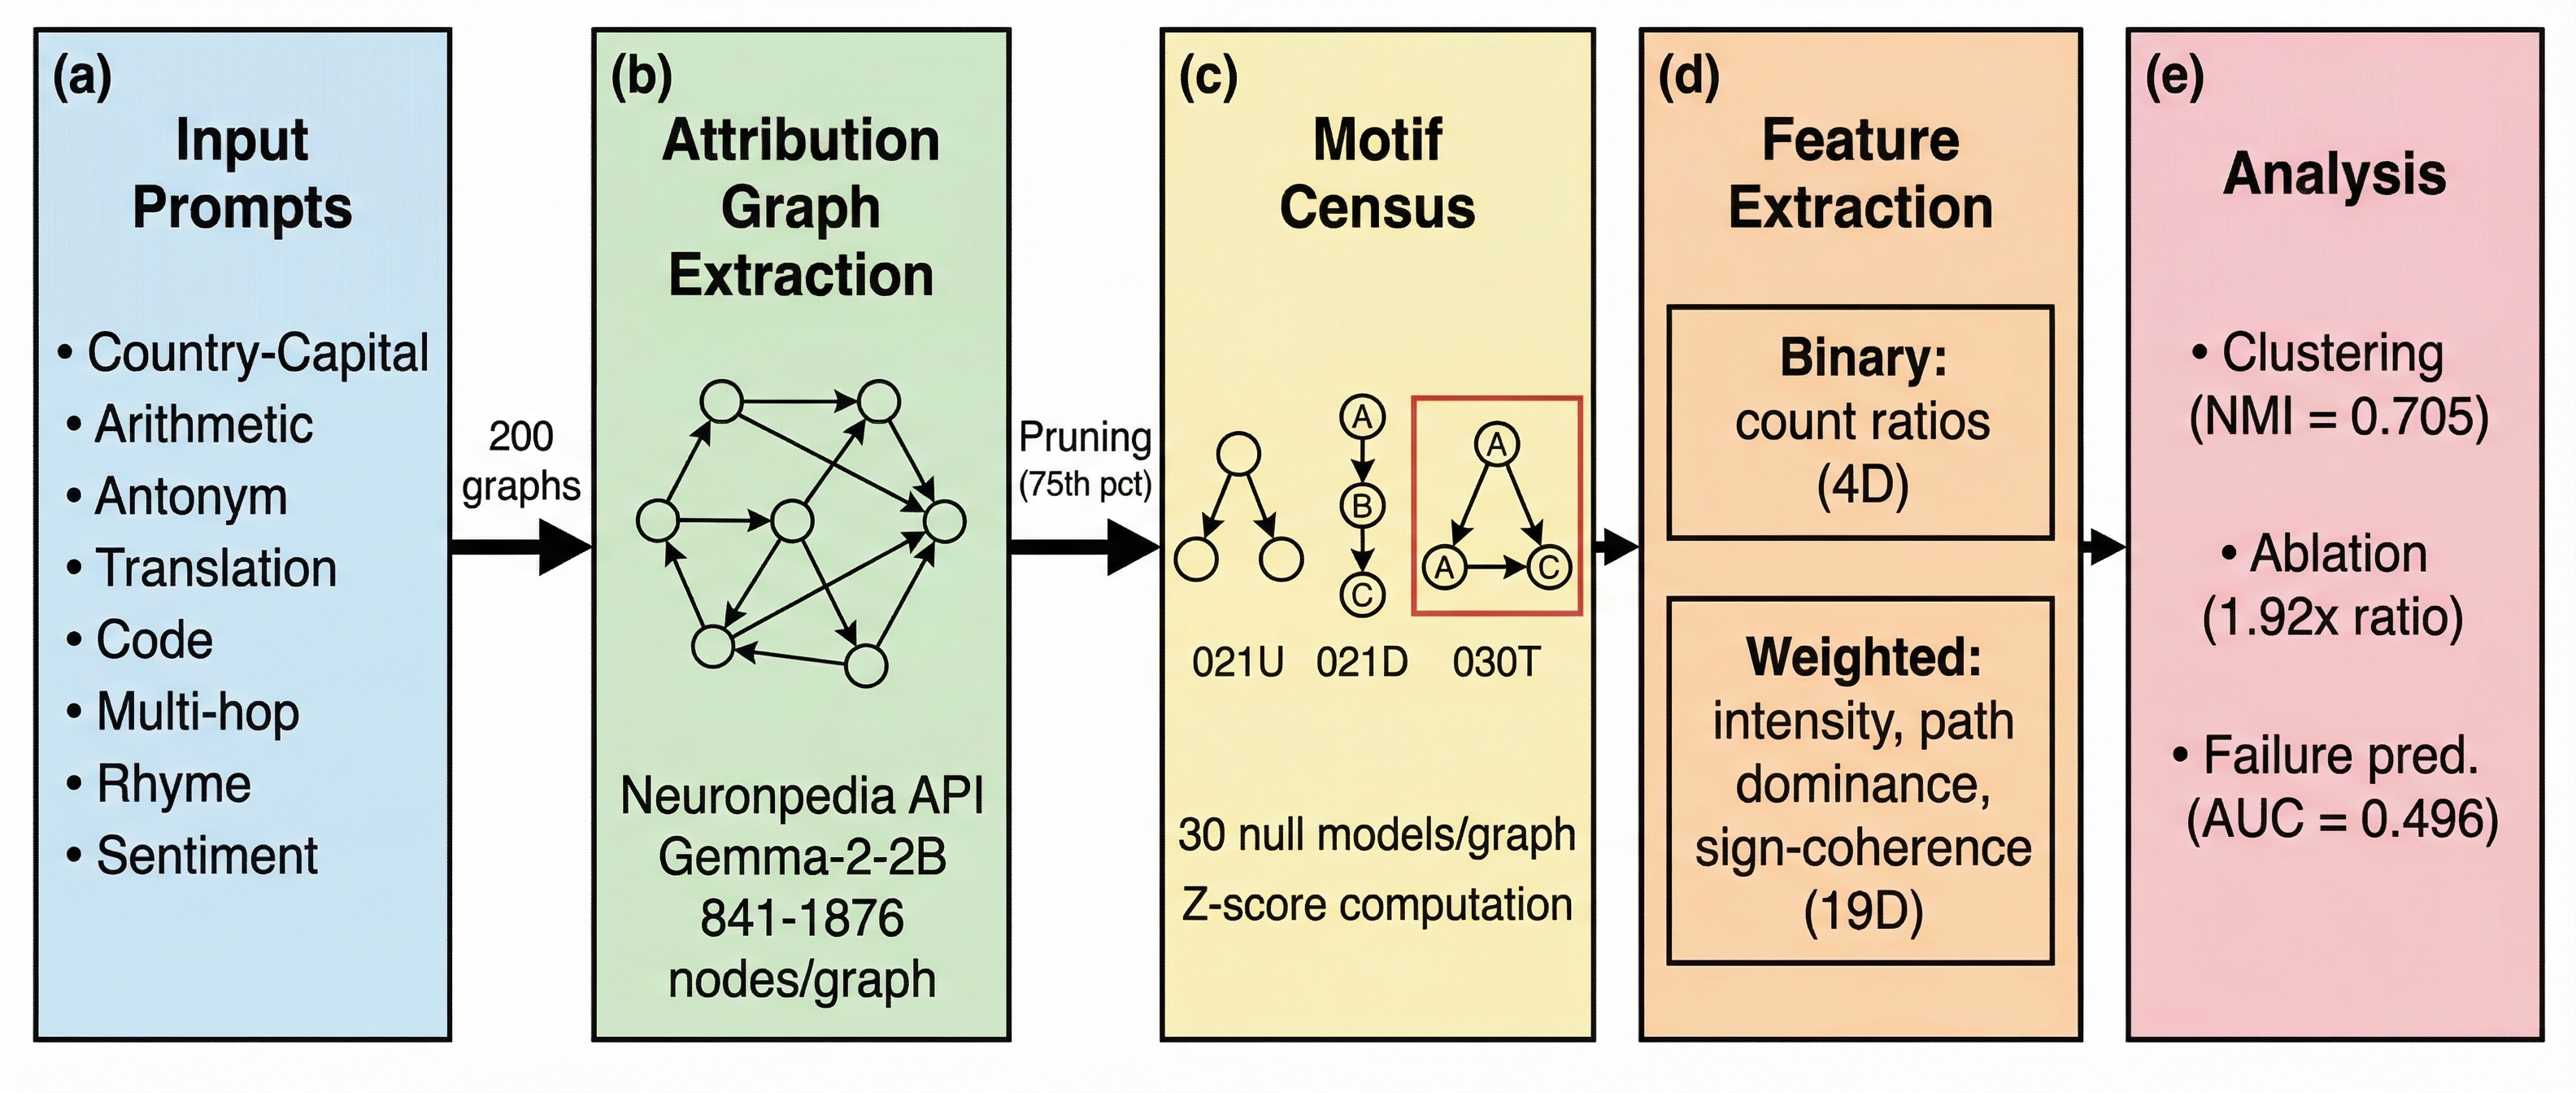
\includegraphics[width=0.92\textwidth,keepaspectratio]{figures/fig_1_v0.png}
  \caption{Overview of the Circuit Motif Spectroscopy framework. (a) Input prompts across 8 capability domains are processed through Gemma-2-2B to generate attribution graphs via Neuronpedia. (b) Each graph undergoes edge pruning (75th percentile) and directed motif census enumeration. (c) Degree-preserving DAG null models are generated via constrained edge swaps, producing Z-scores for each motif type. (d) Weighted motif features (intensity, path dominance, sign-coherence) are extracted from FFL instances. (e) Downstream analyses include capability clustering, graph-theoretic ablation, and failure prediction.}
  \label{fig:pipeline}
\end{figure}

Our analysis yields five principal findings. (1)~The feed-forward loop is massively and universally overrepresented across all 200 graphs and all 8 domains (corpus-level $t$-test: $t = 55.0$, $p = 2.4 \times 10^{-122}$, Cohen's $d = 3.89$), exceeding FFL enrichment in biological networks by 3.7--5.5$\times$. (2)~Weighted motif features cluster circuits by capability domain (NMI $= 0.705$), significantly outperforming binary motif counts (NMI $= 0.101$, $p = 0.001$) and providing unique information beyond graph-level statistics (residualized NMI $= 0.264$, $p = 0.001$). (3)~Graph-theoretic node ablation confirms FFL-hub nodes are structurally critical, causing 1.92$\times$ the downstream attribution disruption of layer-matched controls (CI $[1.91, 1.93]$, $p < 10^{-300}$, Cohen's $d = 0.41$). (4)~Motif spectra do not predict whether the model produces correct outputs (best deconfounded AUC $= 0.496$), an informative negative result. (5)~All four universally overrepresented 4-node motifs exhibit 100\% FFL containment, indicating that LLM circuits organize around a single dominant motif primitive rather than a diverse vocabulary of independent building blocks.

\paragraph{Summary of Contributions.}
\begin{itemize}
  \item We introduce Circuit Motif Spectroscopy, the first application of Alon-style network motif analysis to LLM attribution graphs, bridging systems biology and mechanistic interpretability (Section~\ref{sec:methods}).
  \item We discover that feed-forward loops are universally and massively overrepresented in LLM circuits ($Z \approx 47$, Cohen's $d = 3.89$), exceeding biological benchmarks by 3.7--5.5$\times$, and that all universal 4-node motifs are FFL-derivative (Section~\ref{sec:ffl}).
  \item We demonstrate that weighted motif features (particularly FFL path dominance, $\eta^2 = 0.917$) serve as capability-domain fingerprints carrying unique information beyond graph statistics (Section~\ref{sec:clustering}).
  \item We confirm via graph-theoretic ablation that FFL-hub nodes are disproportionately structurally important (1.92$\times$ layer-matched impact ratio), with a strong dose-response relationship (Spearman $\rho = 0.877$) (Section~\ref{sec:ablation}).
  \item We report an honest negative result: motif spectra cannot predict model failures (AUC $= 0.496$), establishing a boundary on what circuit topology encodes (Section~\ref{sec:failure}).
\end{itemize}

%----------------------------------------------------------------------
\section{Related Work}
\label{sec:related}
%----------------------------------------------------------------------

\paragraph{Network Motifs in Biological and Technological Networks.}
The concept of network motifs was introduced by \citet{Milo2002}, who showed that real-world networks contain small directed subgraph patterns at frequencies significantly exceeding degree-preserving random graph baselines. A subsequent study~\citep{Milo2004} demonstrated that the motif significance profile---the normalized $Z$-score vector across all motif types---classifies networks into superfamilies independent of size or domain. \citet{ShenOrr2002} characterized specific motif functions in \emph{E.~coli} gene regulation, finding that coherent FFLs implement sign-sensitive delay and persistence detection. \citet{Alon2007} systematized these findings into a theory of biological circuit design principles. \citet{Onnela2005} extended motif analysis to weighted networks by defining intensity (geometric mean of edge weights) and coherence metrics. \citet{Saramaki2007} proposed complementary weighted clustering coefficients. These biological network analysis methods form the methodological foundation of our work, applied here to a fundamentally new class of directed causal graphs.

\paragraph{Mechanistic Interpretability and Circuit Discovery.}
The mechanistic interpretability program seeks to understand neural network computations by identifying interpretable features and their causal interactions. \citet{Elhage2021} introduced the mathematical framework for analyzing transformer circuits as compositions of attention heads and MLP layers. The discovery of superposition---where models represent more features than they have dimensions~\citep{Elhage2022}---motivated the development of sparse autoencoders (SAEs) to decompose model activations into interpretable features~\citep{Bricken2023, Cunningham2024, Templeton2024}. Anthropic's circuit tracing work~\citep{Anthropic2025} used SAE-based transcoders to produce attribution graphs for Gemma-2-2B, revealing the causal structure of model computations at the feature level.

Circuit-level analysis has identified specific computational mechanisms: \citet{Wang2023} mapped the indirect object identification circuit in GPT-2, \citet{Nanda2023} tracked progress measures for grokking, and \citet{Meng2022} located factual association storage. \citet{Conmy2023} automated circuit discovery using activation patching. \citet{Marks2024} introduced sparse feature circuits using SAE features and integrated gradients.

\paragraph{Circuit Comparison and Classification.}
Two recent works address circuit comparison but differ fundamentally from our approach. \citet{Sun2025} defined $\alpha$-equivalence for comparing soft circuits via edge overlap, showing that circuit instability correlates with generalization failures. Their metric compares which specific features and edges are shared between circuits, making it identity-dependent---two circuits with entirely different features but similar structural organization would score as dissimilar. Our motif-spectrum approach is identity-agnostic, comparing circuits by their subgraph pattern frequencies regardless of which specific features participate. \citet{Tigges2024} showed circuit components are broadly consistent across Pythia model sizes using node-count correlations, operating at the component level rather than the subgraph pattern level. \citet{Birardi2025} automated attribution graph analysis by clustering features into concept-aligned supernodes, grouping individual features rather than analyzing the graph at the motif level.

No prior work has applied formal Milo/Alon-style network motif analysis---subgraph census, $Z$-scores relative to degree-preserving null models, motif significance profiles, or superfamily classification---to LLM attribution or circuit graphs. This was confirmed through systematic novelty searches across 71+ papers from October 2025 through March 2026.

%----------------------------------------------------------------------
\section{Methods}
\label{sec:methods}
%----------------------------------------------------------------------

\subsection{Attribution Graph Collection}

We collected 200 attribution graphs from the Neuronpedia API (\texttt{POST /api/graph/generate}) using Gemma-2-2B with pre-trained transcoders. Graphs were generated across eight capability domains: country-capital recall (26 graphs), arithmetic addition (26), antonym generation (26), language translation (26), Python code completion (24), multi-hop reasoning (24), rhyme completion (24), and sentiment classification (24). Each prompt was designed to elicit a specific capability (e.g., ``The capital of France is'' for country-capital, ``$7 + 8 =$'' for arithmetic). Raw graphs contained 841--1,876 nodes and 29,000--107,000 directed edges. All 200 graphs were validated as DAGs. Each graph includes correctness annotations indicating whether the model produced the expected output (127 correct, 49 incorrect, 24 unknown).

Nodes in each graph represent four types: input token embeddings, MLP transcoder features, attention transcoder features, and error nodes. Edges carry signed real-valued weights representing the linear causal attribution of one feature's activation on another's.

\subsection{Edge Pruning}

Attribution graphs are dense, containing many low-weight edges that reflect negligible causal effects. Following standard practice, we applied 75th-percentile edge pruning: for each graph, edges with absolute weight below the 75th percentile of absolute edge weights were removed, retaining the top 25\% strongest connections. Pruned graphs contained 841--1,876 nodes (nodes with zero remaining edges were retained). For 4-node motif analysis, which is computationally more expensive, we applied 99th-percentile pruning, retaining 150 of 200 graphs with fewer than 700 nodes post-pruning.

\subsection{Motif Census}

For each pruned graph, we computed the complete directed 3-node motif census using igraph's \texttt{motifs\_randesu()} function, which implements the RAND-ESU algorithm for efficient subgraph enumeration. In DAGs, only 4 of the 13 directed 3-node isomorphism classes can occur: three asymmetric motifs (021U, 021C, 021D in MAN notation---representing fan-out, fan-in, and chain configurations respectively) and the feed-forward loop (030T---where node A connects to both B and C, and B connects to C). For 4-node motifs, 24 of the 199 directed types survive DAG constraints.

\subsection{Null Model Construction}

We generated degree-preserving DAG null models using the Go\~{n}i Method~1 approach~\citep{Goni2014}: iterative random edge swaps that preserve each node's in-degree and out-degree while maintaining acyclicity. Acyclicity was enforced by checking topological ordering after each proposed swap and rejecting swaps that would create cycles. We generated 30 null models per graph for the primary 3-node analysis ($200 \times 30 = 6{,}000$ null graphs) and 20 null models per graph for the 4-node analysis.

For each motif type $i$, the $Z$-score was computed as:
\begin{equation}
  Z_i = \frac{N_{\text{real},i} - \overline{N_{\text{null},i}}}{\sigma(N_{\text{null},i})}
  \label{eq:zscore}
\end{equation}
where $N_{\text{real},i}$ is the count of motif type $i$ in the real graph and $N_{\text{null},i}$ are the counts across null models. Positive $Z$-scores indicate overrepresentation; negative $Z$-scores indicate underrepresentation.

To control for potential confounds from the layered transformer architecture, we additionally generated layer-preserving null models that conserve each node's layer assignment during edge swaps, ensuring that any motif enrichment is not merely an artifact of the layered structure.

\subsection{Weighted Motif Features}

Binary motif counts capture whether a pattern exists but not how attribution flows through motif instances. Following \citet{Onnela2005}, we computed weighted features for each FFL instance ($A \to B$, $A \to C$, $B \to C$):

\begin{itemize}
  \item \textbf{Intensity}: the geometric mean of absolute edge weights, $(|w_{AB}| \cdot |w_{AC}| \cdot |w_{BC}|)^{1/3}$, capturing the overall strength of the motif.
  \item \textbf{Sign-coherence}: the fraction of FFL instances where all three edges share the same sign, indicating whether the direct and indirect paths reinforce or oppose each other.
  \item \textbf{Path dominance}: the ratio $|w_{AB} \cdot w_{BC}| / |w_{AC}|$, measuring the relative strength of the indirect path ($A \to B \to C$) versus the direct path ($A \to C$).
  \item \textbf{Weight asymmetry}: the coefficient of variation of edge weights within each instance.
\end{itemize}

These features were aggregated per graph (mean, median, standard deviation, quartiles) to produce a 19-dimensional weighted motif feature vector alongside the 4-dimensional binary count-ratio vector and an 8-dimensional graph statistics vector (node count, edge count, density, mean degree, max degree, diameter, layer count, mean absolute edge weight).

\subsection{Capability Clustering}

We evaluated whether motif features distinguish capability domains using spectral clustering with varying $K \in \{2, 4, 6, 8\}$. Clustering quality was measured by Normalized Mutual Information (NMI) and Adjusted Rand Index (ARI) against ground-truth domain labels. Statistical significance was assessed via permutation tests (1,000 permutations of domain labels). We compared five feature sets: weighted motif only, binary motif only, graph statistics only, weighted plus binary combined, and all features combined.

To determine whether motif features carry unique information beyond graph-level statistics, we performed McFadden $R^2$ variance decomposition with 1,000 bootstrap resamples, residualized clustering (clustering on motif features after linearly removing graph-statistic dependence via ridge regression), and Canonical Correlation Analysis (CCA).

\subsection{Graph-Theoretic Node Ablation}

To test whether FFL-hub nodes are structurally more important than comparable non-hub nodes, we classified each node by its motif participation index (MPI): the number of FFL instances containing that node. Nodes with MPI above the 90th percentile were classified as FFL-hubs. For each hub node, we identified matched controls using four matching criteria: degree-matched (same total degree $\pm 1$), attribution-matched (same total absolute attribution strength $\pm 10\%$), layer-matched (same layer position), and random (uniformly sampled). Node ablation was simulated by removing the node and all incident edges, then measuring four impact metrics: downstream attribution loss, path disruption, component fragmentation, and reachability reduction. Statistical significance was assessed via paired Wilcoxon signed-rank tests with Benjamini--Hochberg FDR correction.

\subsection{Failure Prediction}

To test whether motif spectra predict model correctness, we trained logistic regression and random forest classifiers on 176 verified graphs (127 correct, 49 incorrect) using stratified 5-fold cross-validation. Feature sets included motif-only, graph-stats-only, domain-only, domain-plus-graph, and a full model combining all features. We computed bootstrap AUC confidence intervals and tested whether adding motif features significantly improved over the domain-plus-graph baseline.

%----------------------------------------------------------------------
\section{Results}
\label{sec:results}
%----------------------------------------------------------------------

\subsection{Universal FFL Overrepresentation}
\label{sec:ffl}

The feed-forward loop (030T) is massively overrepresented in every attribution graph analyzed. Across all 200 graphs, the corpus-level one-sample $t$-test on per-graph $Z$-scores yields $t = 55.0$, $p = 2.38 \times 10^{-122}$, with Cohen's $d = 3.89$---an overwhelmingly large effect. The mean FFL $Z$-score is 47.1 (95\% CI $[45.4, 48.8]$), and the median is 47.8. All 200 graphs show positive FFL $Z$-scores (sign test: $p = 1.24 \times 10^{-60}$), with per-graph values ranging from 16.6 to 81.3.

\begin{figure}[!htbp]
  \centering
  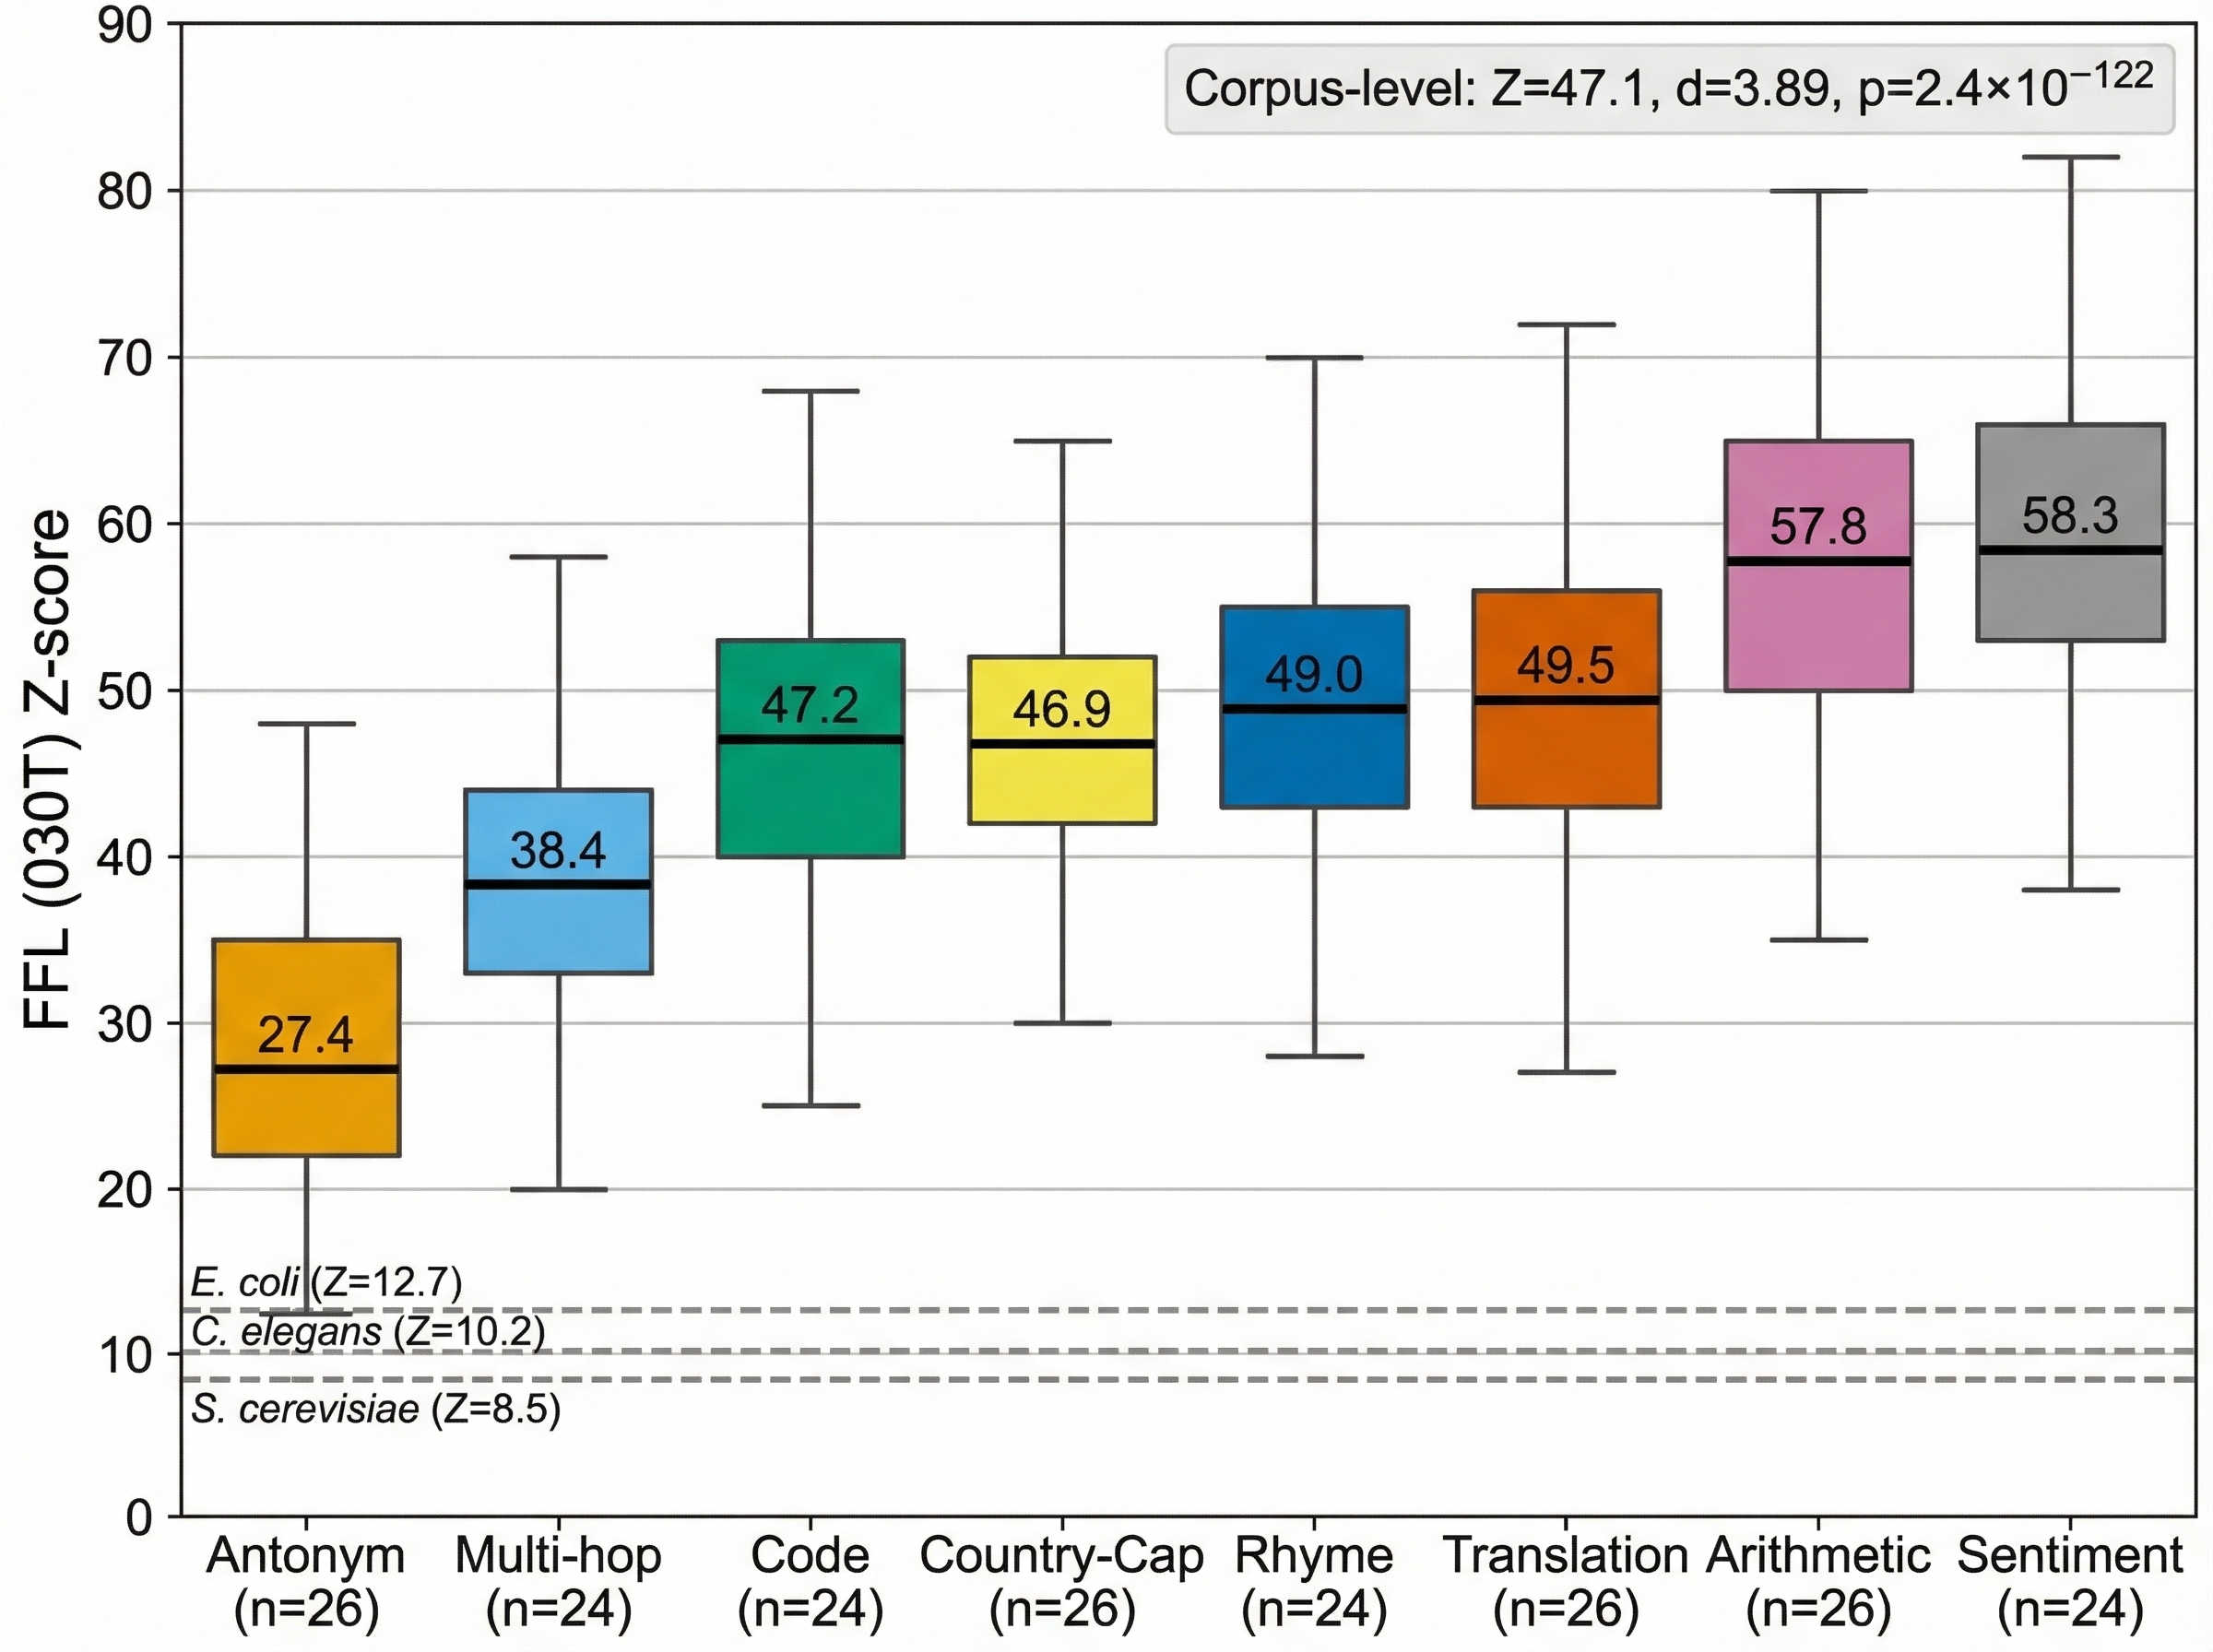
\includegraphics[width=0.92\textwidth,keepaspectratio]{figures/fig_2_v0.png}
  \caption{Distribution of feed-forward loop (030T) Z-scores across 8 capability domains (200 graphs total). Each box shows the interquartile range with median line; whiskers extend to 1.5$\times$ IQR. Dashed horizontal lines indicate FFL Z-scores from canonical biological networks~\citep{Milo2002}. All 200 graphs show positive Z-scores, and all domain medians exceed biological benchmarks by 3.7--5.5$\times$.}
  \label{fig:ffl_zscores}
\end{figure}

FFL overrepresentation is universal across all eight capability domains, though the magnitude varies: sentiment (mean $Z = 59.3$), arithmetic (57.7), translation (49.8), rhyme (48.8), country-capital (47.0), code completion (46.6), multi-hop reasoning (38.5), and antonym (29.8). A linear mixed-effects model with domain as random effect confirms both universality and domain variation: the fixed-effect intercept is $\beta_0 = 47.2$ (95\% CI $[40.5, 53.8]$, $p = 4.9 \times 10^{-44}$), and the intraclass correlation coefficient ICC $= 0.570$ indicates that 57\% of $Z$-score variance is between-domain.

The three non-FFL 3-node motifs (021U, 021C, 021D) are symmetrically underrepresented with mean $Z = -47.1$ in all domains. This perfect antisymmetry arises because, in DAGs, the FFL is the only 3-node motif that can increase in frequency without a proportional decrease in the other three types.

Critically, FFL overrepresentation is not an artifact of the layered transformer architecture. Layer-preserving null models---which additionally conserve each node's layer assignment---produce even higher FFL $Z$-scores (mean $Z = 56.9$ vs.\ 47.1 for degree-preserving nulls), confirming that the signal is genuine.

Comparing to canonical biological networks, LLM attribution graphs exhibit FFL enrichment 3.7$\times$ higher than \emph{E.~coli} transcription regulation ($Z = 12.7$~\citep{Milo2002}), 4.6$\times$ higher than \emph{C.~elegans} neural connectivity ($Z = 10.2$~\citep{Milo2002}), and 5.5$\times$ higher than yeast transcription regulation ($Z = 8.5$~\citep{Milo2002}).

At the 4-node level, 24 directed motif types can occur in DAGs. Of these, four are universally overrepresented (corpus-level Bonferroni-corrected $p < 10^{-22}$ for all four). All four exhibit 100\% FFL containment---every instance of every universal 4-node motif contains at least one embedded 3-node FFL. The universal 4-node motifs are FFL extensions (FFLs with an additional node adding a bypass, relay, or fan-out path), not independent structural primitives.

A critical methodological finding emerged during this analysis: the 3-node motif significance profile (the normalized $Z$-score vector used by \citet{Milo2004} for superfamily classification) is mathematically degenerate under degree-preserving DAG null models. Because DAG constraints heavily restrict which 3-node patterns are possible, the significance profile collapses to a near-constant vector $[-0.5, -0.5, -0.5, 0.5]$ for every graph. The elegant Milo/Alon superfamily classification via significance profile cosine similarity therefore does not directly apply at the 3-node level for DAGs. The 4-node significance profile has higher effective dimensionality (14 dimensions), partially rescuing the framework.

\subsection{Capability Clustering via Motif Spectra}
\label{sec:clustering}

Weighted motif features cluster attribution graphs by capability domain substantially better than binary motif counts. Spectral clustering at $K = 8$ (matching the number of domains) achieves NMI $= 0.705$ with weighted motif features, compared to NMI $= 0.101$ for binary motif count ratios---a 7$\times$ improvement (permutation $p = 0.001$). Weighted motif features also outperform graph-level statistics (NMI $= 0.677$ at $K = 4$, permutation $p = 0.001$). Combining all feature sets yields NMI $= 0.844$ ($K = 8$, ARI $= 0.688$), indicating substantial complementarity.

\begin{figure}[!htbp]
  \centering
  \includegraphics[width=0.92\textwidth,keepaspectratio]{figures/fig_3_v0.png}
  \caption{t-SNE embeddings of 200 attribution graphs colored by capability domain, comparing four feature sets. (a) Binary motif count ratios fail to separate domains (NMI $= 0.101$). (b) Graph-level statistics provide moderate separation (NMI $= 0.677$). (c) Weighted motif features achieve strong clustering (NMI $= 0.705$). (d) Combining all features yields the best separation (NMI $= 0.844$). Points represent individual attribution graphs; colors indicate capability domains.}
  \label{fig:clustering}
\end{figure}

The most discriminative individual feature is FFL path dominance---the ratio of indirect-path to direct-path attribution weight---with $\eta^2 = 0.917$ (one-way ANOVA, $F = 302.9$, $p = 4.0 \times 10^{-100}$). Path dominance varies systematically across domains: sentiment circuits show the highest mean path dominance (1.99), indicating that indirect FFL paths dominate over direct paths, while arithmetic circuits show the lowest (0.72), indicating direct-path dominance. FFL intensity ($\eta^2 = 0.810$), fan-in intensity ($\eta^2 = 0.842$), and fan-out intensity ($\eta^2 = 0.823$) are also strongly discriminative.

\begin{figure}[!htbp]
  \centering
  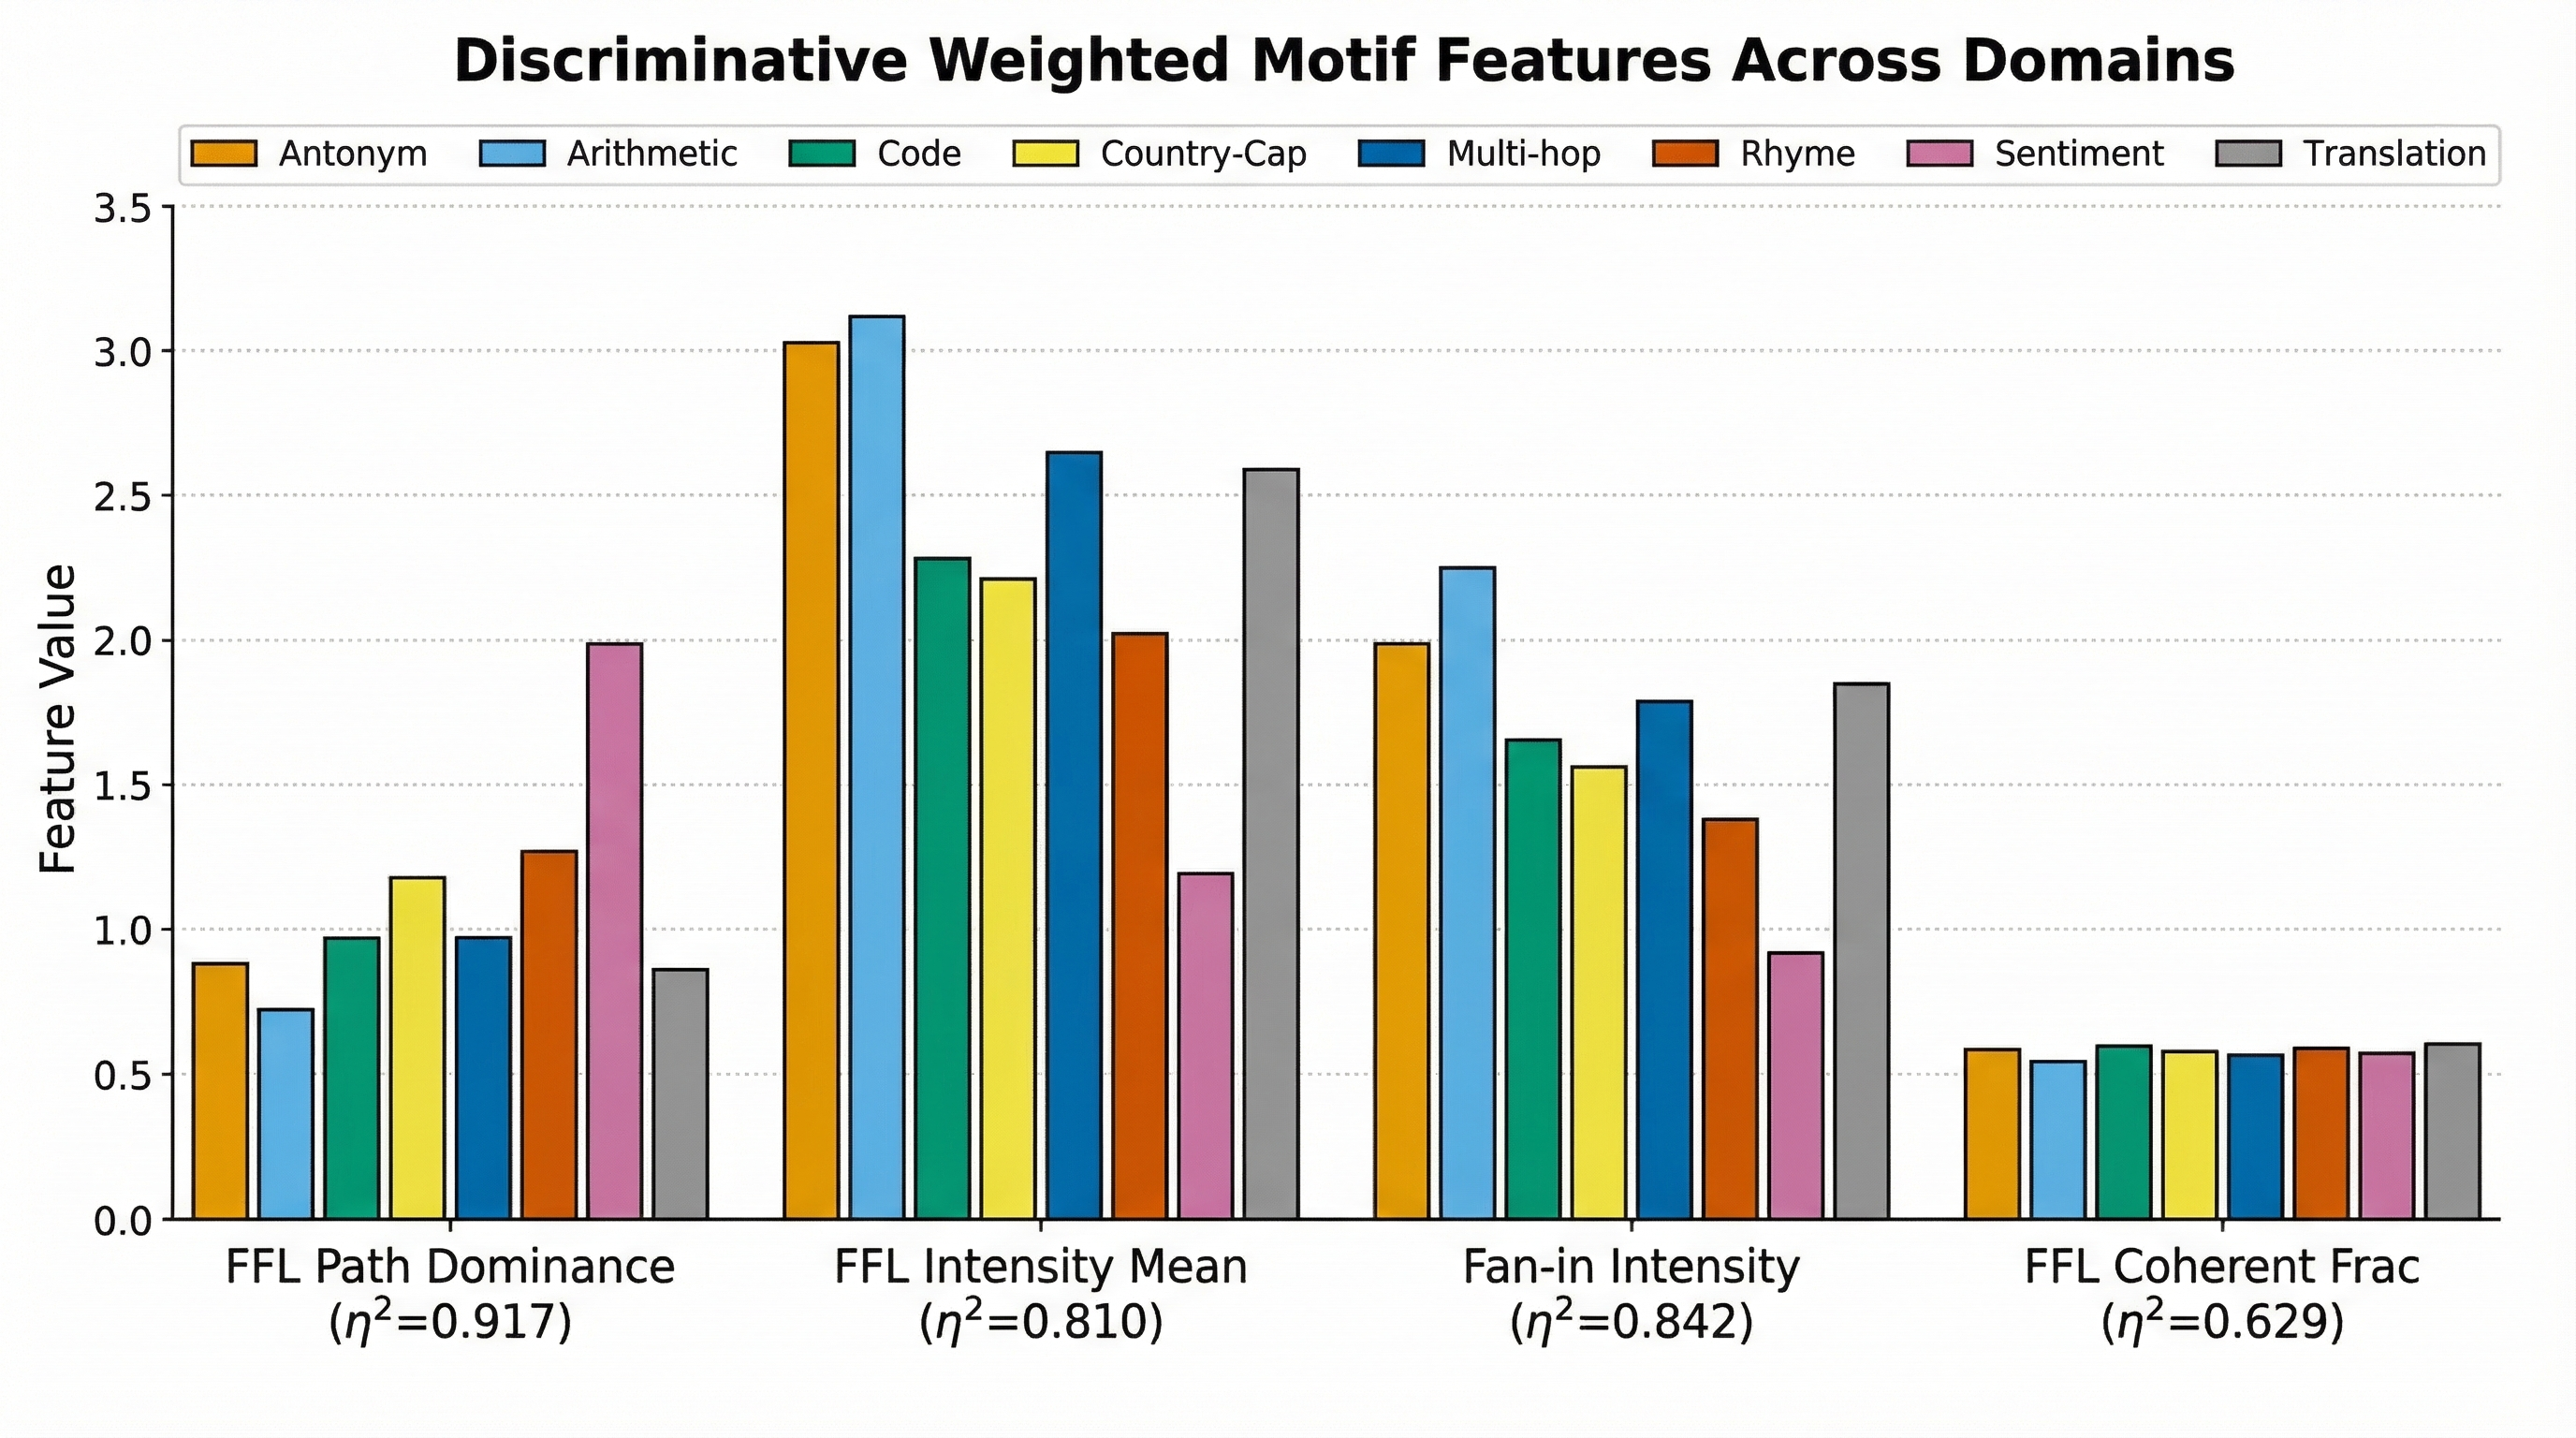
\includegraphics[width=0.92\textwidth,keepaspectratio]{figures/fig_4_v0.png}
  \caption{Mean values of the four most discriminative weighted motif features across 8 capability domains, with ANOVA $\eta^2$ values indicating effect size. FFL path dominance ($\eta^2 = 0.917$) shows the greatest domain discrimination: sentiment circuits favor indirect FFL paths (mean $= 1.99$) while arithmetic circuits favor direct paths (mean $= 0.72$).}
  \label{fig:features}
\end{figure}

\paragraph{Unique Information Beyond Graph Statistics.}
A variance decomposition analysis quantifies the unique information contributed by motif features. McFadden $R^2$ decomposition with 1,000 bootstraps yields: shared variance $= 0.930$, unique graph-statistics $= 0.050$, and unique motif $= 0.018$ (bootstrap CI excluding zero). Residualized clustering---spectral clustering on motif features after linearly removing all graph-statistic dependence via ridge regression---achieves NMI $= 0.264$ (permutation $p = 0.001$), confirming that motif features capture genuine structural information that graph-level statistics cannot.

\begin{figure}[!htbp]
  \centering
  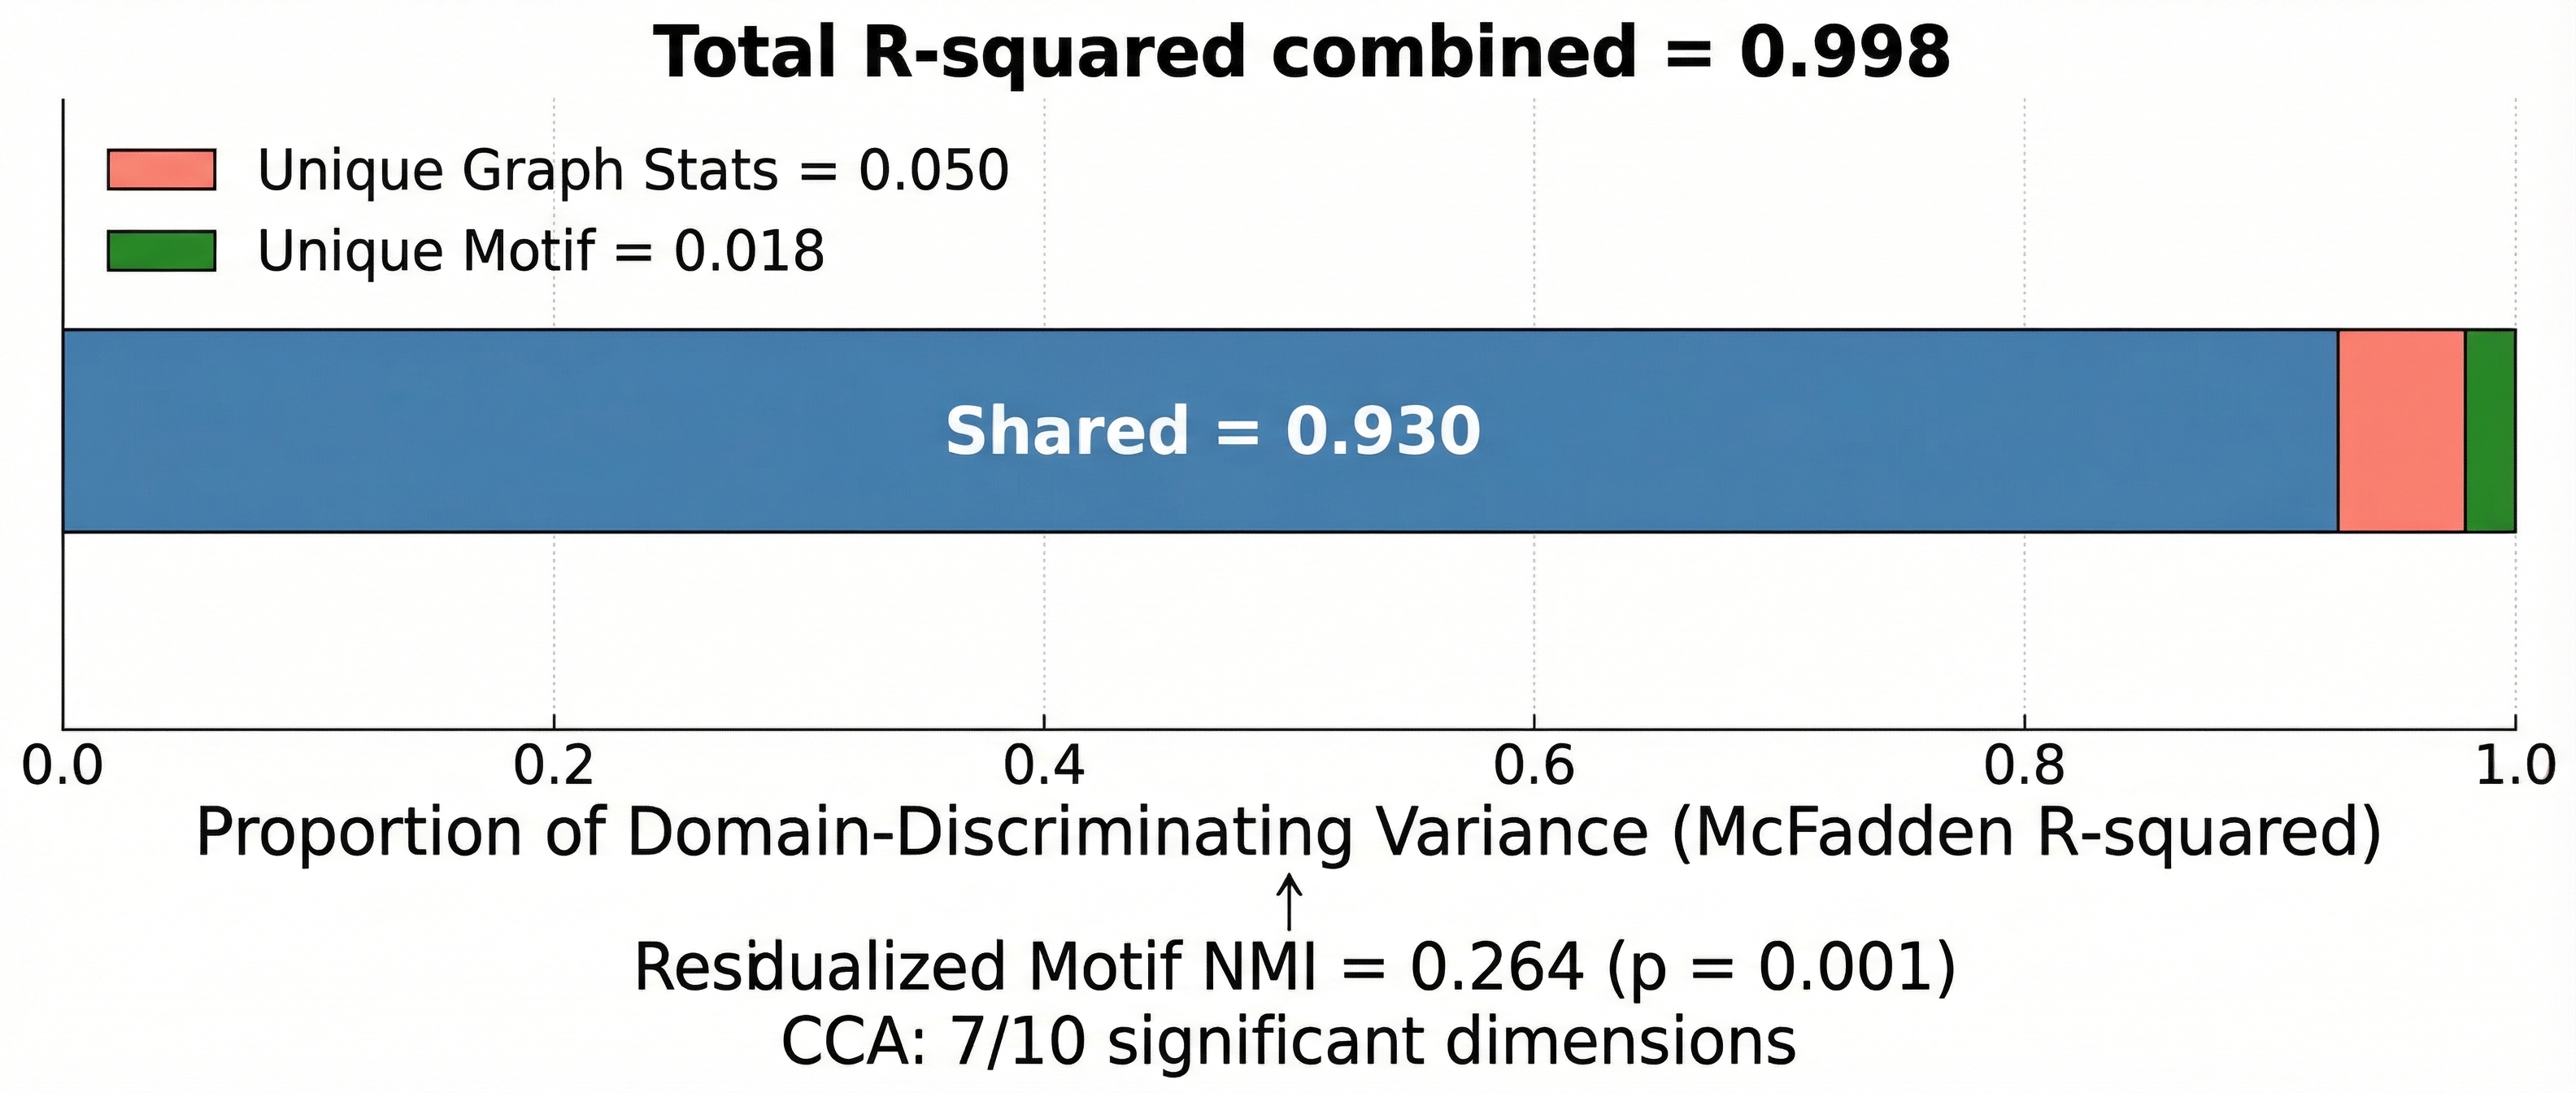
\includegraphics[width=0.92\textwidth,keepaspectratio]{figures/fig_5_v0.png}
  \caption{McFadden $R^2$ variance decomposition showing the proportion of domain-discriminating information attributable to motif features, graph-level statistics, and their shared component. Motif features carry a small but statistically significant unique contribution ($R^2 = 0.018$, bootstrap CI excluding zero), while 93.0\% of the information is shared between the two feature sets.}
  \label{fig:variance}
\end{figure}

Canonical Correlation Analysis finds 7 of 10 canonical dimensions significantly correlated between motif and graph-statistic feature spaces, confirming substantial but incomplete overlap. The retained mutual information after residualization is 23.6\%, indicating that roughly one-quarter of the domain-discriminating information in motif features is orthogonal to graph-level statistics.

\subsection{Structural Importance of FFL-Hub Nodes}
\label{sec:ablation}

Graph-theoretic node ablation across all 200 graphs confirms that nodes heavily participating in FFL motifs are disproportionately structurally important. We enumerated 11.2 million FFL instances and classified 20,056 nodes (7.94\% of all nodes) as FFL-hubs (90th percentile of motif participation).

\begin{figure}[!htbp]
  \centering
  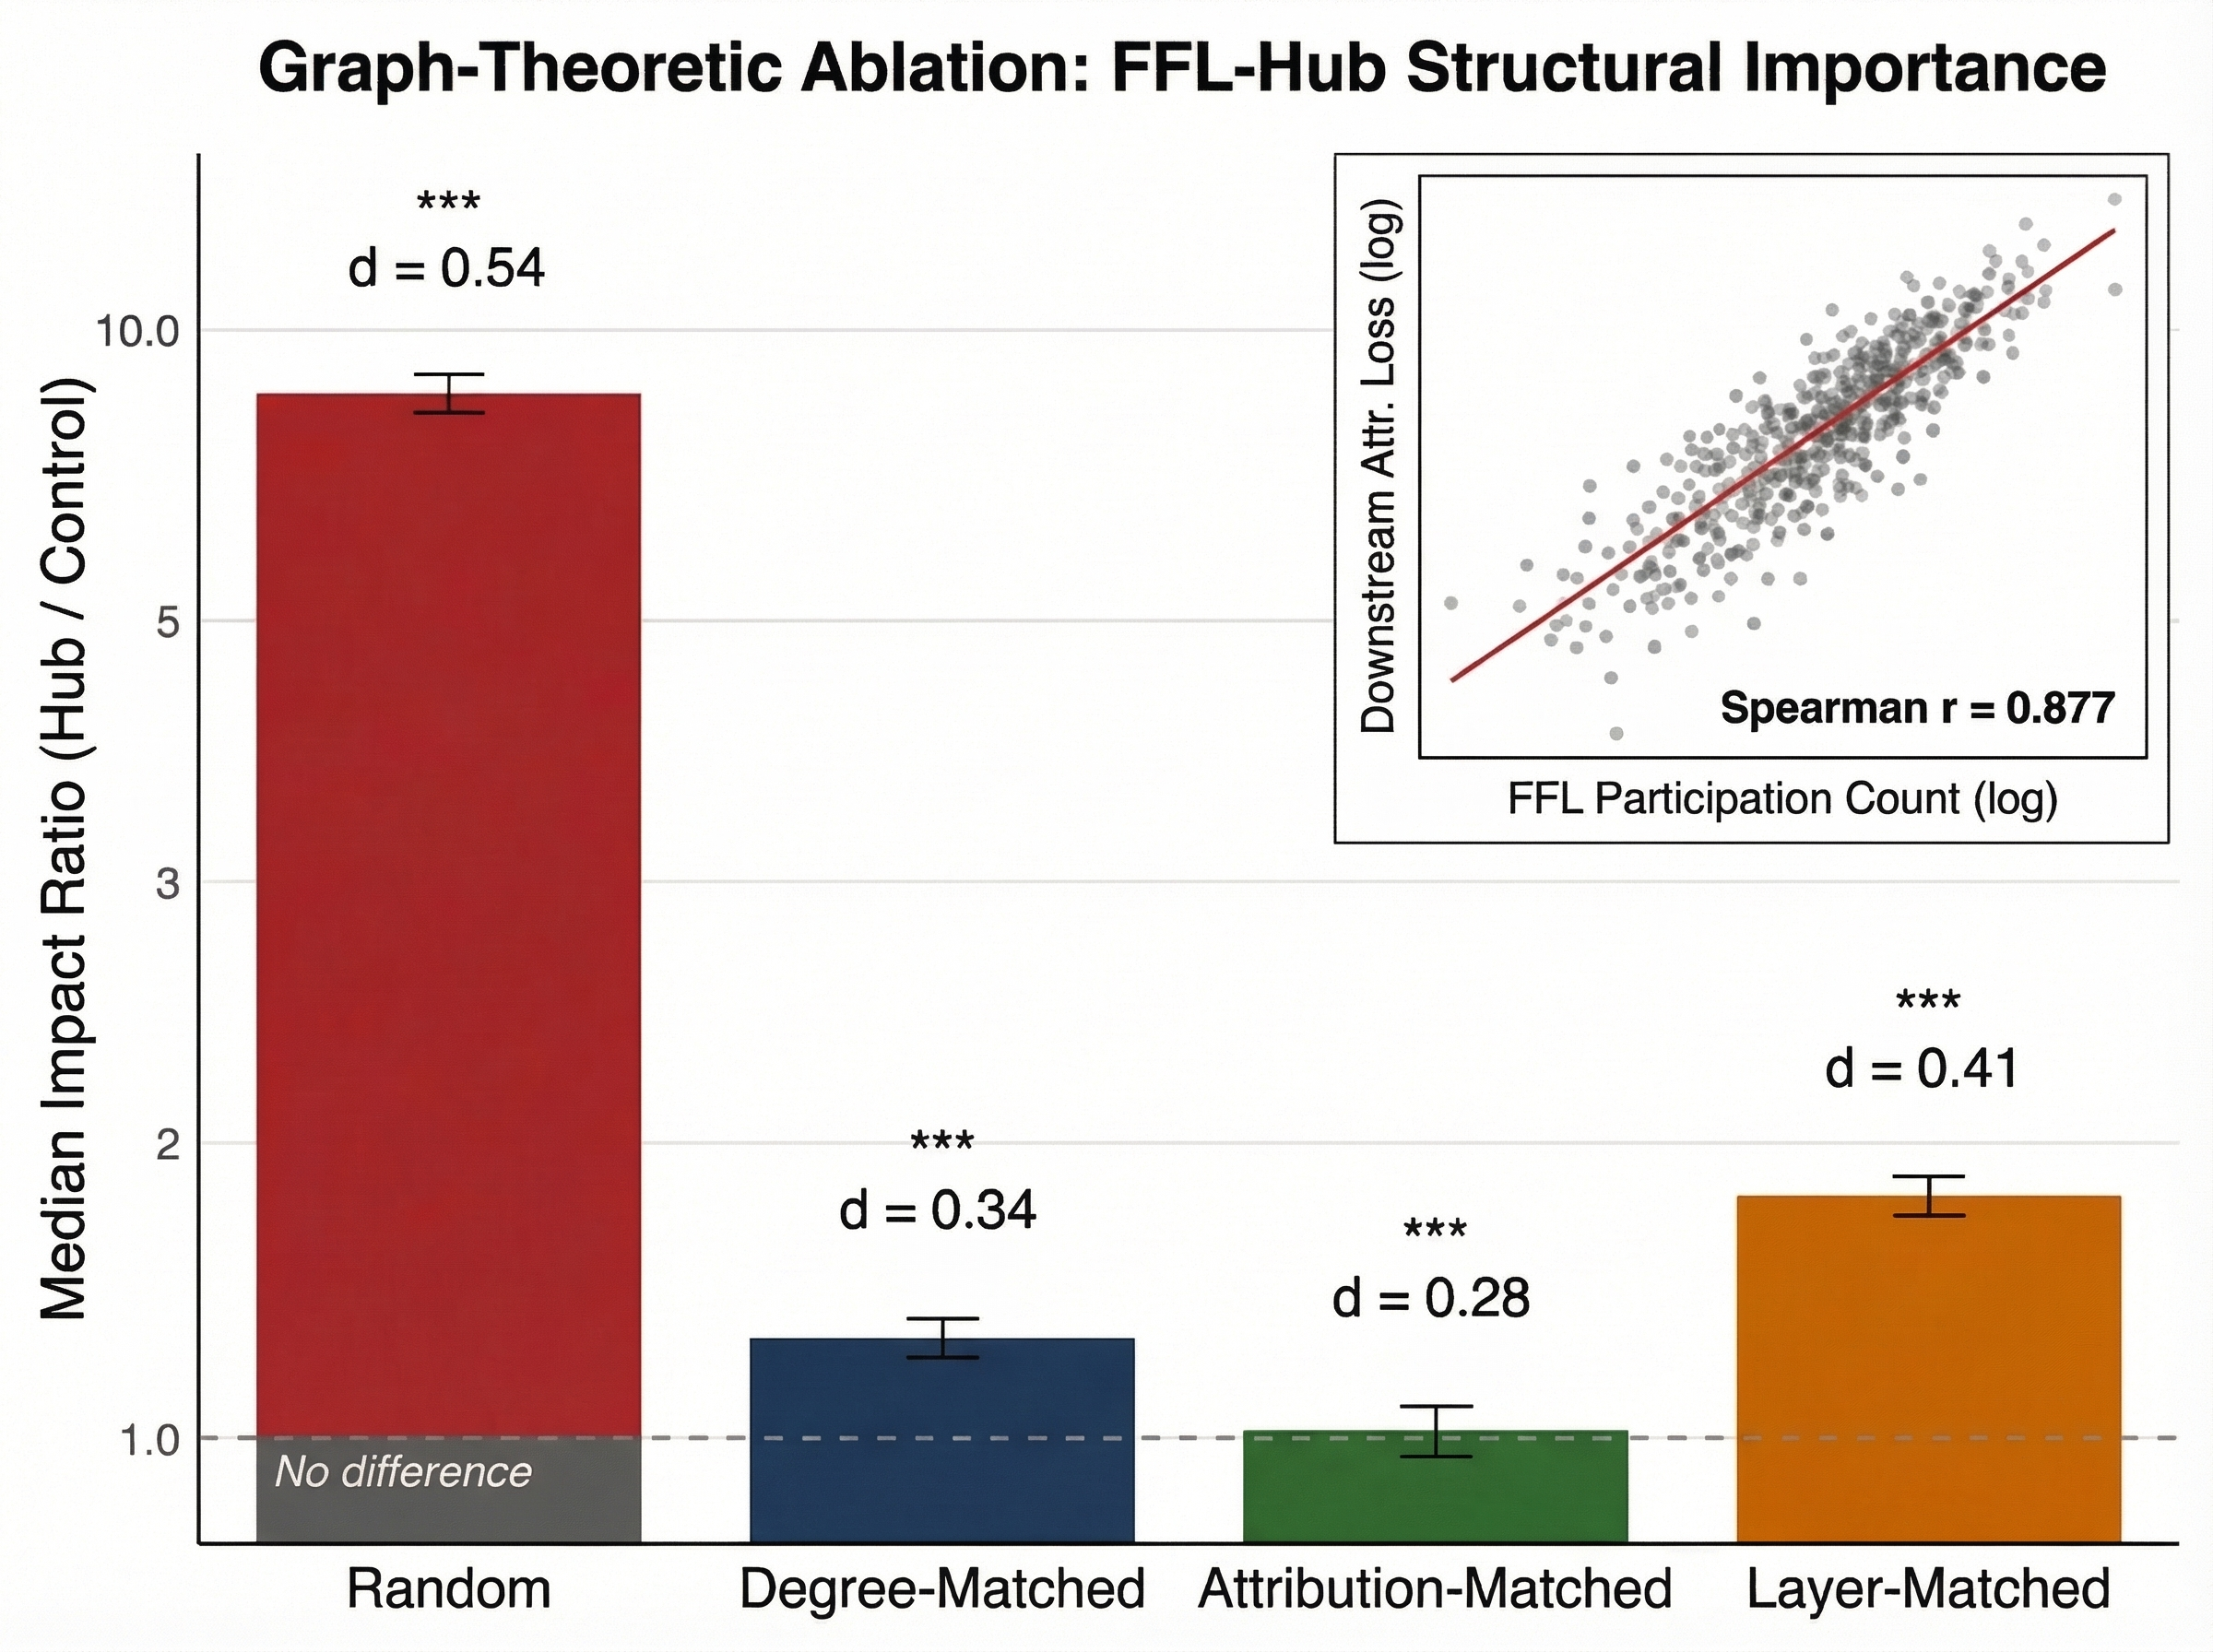
\includegraphics[width=0.92\textwidth,keepaspectratio]{figures/fig_6_v0.png}
  \caption{Median downstream attribution loss ratio (FFL-hub nodes / matched control nodes) across four matching conditions. FFL-hub ablation causes 1.92$\times$ the disruption of layer-matched controls and 9.23$\times$ the disruption of random controls (all $p < 10^{-300}$). Inset: dose-response relationship between FFL participation count and downstream attribution loss (Spearman $\rho = 0.877$).}
  \label{fig:ablation}
\end{figure}

FFL-hub ablation produces significantly greater downstream attribution loss than all four types of matched controls. Against the most stringent baseline---layer-matched controls (same layer position)---FFL-hubs cause 1.92$\times$ the median downstream attribution loss (95\% CI $[1.91, 1.93]$, Wilcoxon $p < 10^{-300}$, Cohen's $d = 0.41$). Against random controls, the ratio reaches 9.23$\times$ (Cohen's $d = 0.54$). Against degree-matched controls, the ratio is 1.35$\times$, and against attribution-matched controls, 1.02$\times$. The diminishing ratio with more stringent matching isolates the FFL-specific contribution: even after controlling for degree, layer, and attribution strength, FFL participation confers additional structural importance.

A dose-response analysis reveals a strong monotonic relationship between FFL participation count and downstream impact: Spearman $\rho = 0.877$ for downstream attribution loss versus motif participation index. Nodes participating in more FFLs are progressively more structurally important. All eight domains show significant effects ($p < 0.05$ after FDR correction).

\subsection{Failure Prediction: An Informative Negative}
\label{sec:failure}

We tested whether motif spectral deviations predict model errors using deconfounded classifiers on 176 verified graphs (127 correct, 49 incorrect). The result is cleanly negative: motif-only features achieve AUC $= 0.496$ (below chance), while the best overall model (graph-statistics-only logistic regression) achieves AUC $= 0.583$ (bootstrap 95\% CI $[0.484, 0.668]$). Adding motif features to the domain-plus-graph baseline provides no significant lift (AUC difference $= -0.020$, $p = 0.865$).

This negative result is informative rather than disappointing. An earlier analysis without domain deconfounding had yielded AUC $= 0.853$, but internal statistical auditing revealed this was driven by domain confounding: different domains have both different correctness rates and different motif spectra. After deconfounding, the signal vanishes. Circuit topology encodes \emph{what kind} of computation is being performed (which domain), not \emph{how well} the computation is being performed (whether the answer is correct). Failure likely depends on feature-level semantics, activation magnitudes, or factors invisible to structural motif analysis.

\subsection{FFL Functional Characterization}
\label{sec:functional}

Enumeration of 1.9 million FFL instances across 34 detailed-analysis graphs reveals striking structural regularities. All FFLs (100\%) exhibit strict layer ordering: node A resides at an earlier layer than B, and B at an earlier layer than C. By contrast, only 35\% of random connected triads show strict layer ordering ($\chi^2 = 1.17 \times 10^{6}$, $p \approx 0$, Cram\'{e}r's $V = 0.32$). FFLs in attribution graphs are not arbitrary triangular connections but specifically implement feed-forward computational cascades spanning multiple transformer layers.

Among enumerated FFLs, 58\% are coherent---the direct path ($A \to C$) and indirect path ($A \to B \to C$) have the same sign, meaning both paths reinforce the same effect on node C. This is consistent with the biological literature, where coherent FFLs implement persistence detection and noise filtering~\citep{ShenOrr2002, Alon2007}. However, cross-domain semantic consistency of FFL node roles is weak (Cram\'{e}r's $V = 0.13$), indicating that FFLs do not consistently map the same semantic categories to the same structural positions across different capability domains.

%----------------------------------------------------------------------
\section{Discussion}
\label{sec:discussion}
%----------------------------------------------------------------------

\paragraph{The FFL as a Universal Computational Primitive.}
The central finding of this work---that the feed-forward loop is the sole universally overrepresented motif in LLM attribution graphs---has both expected and surprising aspects. The existence of FFLs was anticipated from Anthropic's case studies~\citep{Anthropic2025}, which noted parallel direct and indirect paths (e.g., ``Dallas'' $\to$ ``Austin'' directly and ``Dallas'' $\to$ ``Texas'' $\to$ ``Austin'' indirectly). What was not anticipated was (a)~the overwhelming magnitude of overrepresentation ($Z \approx 47$, compared to $Z = 8$--$13$ in biological networks), (b)~the universality across all eight tested capability domains, and (c)~the absence of other universally overrepresented independent motifs---all universal 4-node motifs are FFL extensions.

The FFL's prevalence in LLM circuits likely reflects a fundamental computational strategy: establishing parallel direct and indirect information pathways that enable both redundancy (protecting against single-path failures) and hierarchical processing (the indirect path can perform additional transformation). The high coherence rate (58\%) suggests that the majority of FFLs implement reinforcing rather than inhibiting indirect paths.

\paragraph{Weighted Features as Capability Fingerprints.}
The striking contrast between binary motif clustering (NMI $= 0.101$) and weighted motif clustering (NMI $= 0.705$) reveals that the topology of attribution graphs is largely domain-invariant---all domains use FFLs---but the quantitative flow of attribution through FFLs varies systematically by domain. FFL path dominance ($\eta^2 = 0.917$) is the key discriminant: arithmetic circuits route attribution primarily through direct paths (mean path dominance $= 0.72$), while sentiment circuits favor indirect paths (mean path dominance $= 1.99$). This suggests that different computational tasks require different balances between direct feature interaction and mediated, multi-step processing.

\paragraph{Comparison to Biological Networks.}
LLM attribution graphs exhibit FFL enrichment 3.7--5.5$\times$ higher than canonical biological networks. This disparity may reflect fundamental differences in how these networks are constructed. Biological networks evolved under noise, energy constraints, and selection pressures that favor robust but minimally complex solutions. LLM circuits, by contrast, emerged from gradient-based optimization on vast data, without explicit pressure toward parsimony. The extreme FFL overrepresentation in LLMs may indicate that gradient descent, when operating on densely connected layered architectures, converges on FFL-heavy solutions as a natural consequence of optimization dynamics.

The mathematical degeneracy of the 3-node significance profile under DAG constraints is a methodological contribution with implications beyond this study. Any future application of motif analysis to layered DAGs---including other neural network circuit analyses---must account for this constraint. The 4-node level provides richer discriminative structure (14 effective dimensions vs.\ 1), and we recommend 4-node analysis as the minimum for superfamily-style classification in DAG networks.

\paragraph{Limitations.}
Several limitations constrain the generalizability of these findings. First, all 200 graphs come from a single model (Gemma-2-2B) via a single circuit extraction method (Neuronpedia transcoders). Whether FFL dominance generalizes to other architectures (Llama, GPT-family, Mamba), larger models, or alternative circuit extraction methods (activation patching, causal scrubbing) is untested. Second, the graph-theoretic ablation proxy demonstrates structural importance but does not prove that removing an FFL-hub node from the live model changes the model output; real model-level causal interventions were infeasible due to API limitations. Third, the unique variance contributed by motif features beyond graph statistics is real but modest ($R^2 = 0.018$), meaning that approximately 93\% of what motifs tell us about domain identity is also encoded in simpler statistics. Fourth, the correctness annotations are based on automated checking, and the class imbalance (127 correct vs.\ 49 incorrect) may limit statistical power for failure prediction. Fifth, the motif framework treats all edges as equally important regardless of their position in the computational graph, potentially missing hierarchical structure.

%----------------------------------------------------------------------
\section{Conclusion}
\label{sec:conclusion}
%----------------------------------------------------------------------

We introduced Circuit Motif Spectroscopy, the first systematic application of biological network motif analysis to LLM attribution graphs. Across 200 graphs from Gemma-2-2B spanning eight capability domains, we established that (1)~the feed-forward loop is a universal, massively overrepresented computational building block ($Z = 47.1$, $d = 3.89$, $p = 2.4 \times 10^{-122}$), (2)~weighted motif features fingerprint circuits by capability domain (NMI $= 0.705$) with unique information beyond graph statistics (residualized NMI $= 0.264$), (3)~FFL-hub nodes are disproportionately structurally important (1.92$\times$ layer-matched ablation ratio), and (4)~circuit topology encodes computation type but not computation success (failure prediction AUC $= 0.496$).

These findings suggest deep structural parallels between biological and artificial information-processing systems---both converge on feed-forward loop motifs as fundamental computational primitives, despite radically different construction mechanisms. Future work should extend the analysis to multiple model architectures, perform real model-level causal interventions on motif nodes, investigate whether motif structure changes across training, and explore whether motif-aware circuit pruning can improve model efficiency.

\bibliography{references}

\end{document}
